\p
ابتدا نشان دهید برای هر دو راس از
$6n + 1$
ضلعی منتظم مانند
$A$
و
$B$
دقیقا سه راس مانند
$C$
وجود دارد به‌طوری که
$ABC$
مثلثی متساوی‌الساقین باشد و نتیجه بگیرید تعداد مثلث‌های متساوی‌الساقین که رئوس هر یک از بین راس‌های
$6n + 1$
ضلعی باشد، برابر
$t = 3n(6n + 1)$
است. فرض کنید در
$r$
تا از این مثلث‌ها هر سه راس هم‌رنگ باشند. این مثلث‌ها را با
$T_1, \cdots, T_r$
و بقیه را با
$T_{r+1}, \cdots, T_t$
نشان می‌دهیم. جدولی
$k(6n + 1 - k) \times t$
تشکیل می‌دهیم که هر سطر آن متناظر با یک جفت راس که یکی قرمز و یکی آبی است و هر ستون آن متناظر با یکی از
$T_i$
ها باشد. اگر
$A$
راسی قرمز و
$B$
راسی آبی از مثلث
$T_i$
باشد، در این صورت در خانه‌ی محل تقاطع سطر متناظر با
$A$
و
$B$
و ستون متناظر با
$T_i$
عدد
$1$
و در غیر این صورت عدد صفر را قرار می‌دهیم. مجموع اعداد هر سطر از این جدول برابر
$3$
، مجموع اعداد هر یک از ستون‌های متناظر با
$T_1, \cdots, T_r$
برابر صفر و مجموع اعداد هر یک از ستون‌های متناظر با
$T_{r+1}, \cdots, T_t$
برابر
$2$
است. نتیجه می‌گیریم:
$$3k(6n + 1 - k) = 2(t - r) \Rightarrow 2r = 2t - 3k(6n + 1 - k)$$
$$= 6n(6n + 1) - 3k(6n + 1 - k)$$
\begin{center}
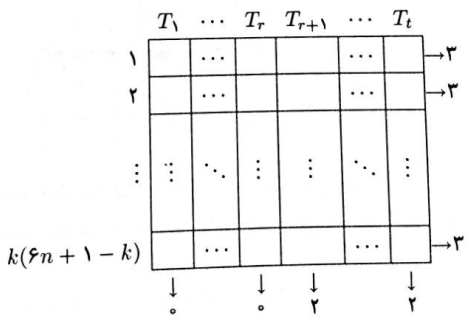
\includegraphics[height=6.5cm]{1.png}
\end{center}
لذا
$r$
فقط به
$n$
و
$k$
بستگی دارد.